\documentclass[11pt]{article}
\usepackage[margin=0.7in]{geometry}
\newcommand{\ts}{\textsuperscript}
%Gummi|065|=)
\date{}

%%%%% Please Check this section %%%%%
\title{Table of Contents}

\usepackage{graphicx}
\begin{document}

%% This is Final Report for MSE 110
%	Must be single spaced which I think it is right
%	Printed on BOTH pages
%	Include a listing of the program 
%	Submit all the project files on canvas
%	Use the cover paper provided on canvas (I made the file)
%	include a link to the project demonstration video (Maybe use youtube or google drive

%% Structure of the report (Refer to the document 'Final Project Report Instruction.pdf')
%	Progress section
%	Mechanical Design
%	Software Design 


\maketitle

\tableofcontents

\newpage


\section{Progress Report}
\subsection{1\ts{st} Iteration}

Should be achieved by:
\begin{itemize}
\item Robot moves forward exactly one cell length and turns 90 $^{\circ}$ accurately\\
This is the most important feature of our robot. By ensuring accurate movement, we limit the need to readjust in each cell.
\item Robot follows right wall\\
This is the algorithm needed to find the unique solution to the maze. Once movement is implemented, we can just build on top of it to collect more data as we move through the maze. 
\end{itemize}

\subsection{2\ts{nd} Iteration}

Should be achieved by:
\begin{itemize}
\item Robot tracks its orientation and location in maze\\
This is dependency for most of the other requirements. By tracking movement in the cell, we are able to know when we have reached our goal and where to store cell information in our 2-D array.
\item Robot beeps when reached target
\item Robot stores wall information, visited/unvisited status and orientation at entry in 2-D array.\\
This is required for more advanced algorithm features we wish to implement such as having the robot not check the same wall twice and displaying current location and wall information graphically. However, we chose to implement it now because it was a major criteria requirement. 
\end{itemize}

\subsection{3\ts{rd} Iteration}

Should be achieved by:
\begin{itemize}
\item Robot returns with shortest path\\
Since we know the route we took to get to our final location, we can now implement the cancelling algorithm (described in detail at \textbf{section 3.16}).
\item Robot displays current location graphically on screen\\
We implemented this now so that we could more easily test our algorithm. The last project feature we wanted to implement was to not check the same wall twice. We thought that this would be difficult to implement and as such improved our debugging capabilities before continuing.
\end{itemize}

\subsection{4\ts{th} Iteration}
Should be achieved by:

\begin{itemize}
\item Improve algorithm such that robot doesn't check same wall twice\\
The premise behind this optimization is that imagine that we are in a cell with a wall to the South. If we've checked that there is a wall toward the south, we know that in the cell below our current cell, there is a wall to the North. The most general case will be programmed and described in section 3. This has two major advantages: we do not have to waste time turning and we do not incur extra error because of unneeded turning.
\end{itemize}

\newpage
\section{Mechanical Design of MazeBot}
\subsection{Top Level Mechanical Structure and Specifications}
Our robot needed very accurate movement in order to be successful in the maze. This criteria depends heavily on whether or not the motor encoders report accurate values to the algorithm. In order to achieve this, we had to ensure:

\begin{itemize}
\item The wheels do not slip
\item The robot does not hit walls
\item The drive system is sturdy 
\item The gears are securely held in place and make proper contact. 
\end{itemize}
However, there is a limit to how much we can to do minimize mechanical error in movement. As a result, we will have to readjust after a certain number of cells. This is done by driving into the wall, turning 90$^{\circ}$ and driving into the wall again. However, having to readjust too often is problematic as this adds time to our average time in each cell which is a major criteria point. As a result, we hope to minimize the amount of times we need to readjust by maximizing the accuracy of the mechanical system. 

\newpage

\subsection{First Iteration}
\textbf{Goals:}
\begin{itemize}
\item Able to go 3 cells without needing to readjust
\item Able to turn 90$^{\circ}$ accurately.
\end{itemize}
\textbf{Mechanical Drawing}\\

\underline{\textbf{Observations \& Measurements}}\\\\
\textbf{Goal}: Able to go 3 cells without needing to readjust\\
\textbf{Failed}: Needed to readjust every second cell\\\\
\textbf{Goal}: Able to turn 90$^{\circ}$ accurately.\\
Test - An error of even $ \pm 1^{\circ}$ will cause accumulate to a significant error when traversing cells. However, error in turning is hard to notice. Therefore, we chose to have robot turn 90$^{\circ}$ 8 times in place in order to propogate any error significantly. \\
\textbf{Failed}: Robot had error of $ \pm 20^{\circ}$\\\\
\textbf{\underline{Reasons for Test Failures:}}\\
\textbf{Structural Integrity of the Drive System}\\
In order for more accurate movement, we added a high gear ratio. However, since we added the high gear ratio, we are unable to find space to properly secure the left and right drive wheels. When testing, we found one wheel to slipped forward and the other to slipped back when turning which defeats the accuracy of the encoder. Because of this, we are unable to meet our goal of accurate movement.\\\\
\textbf{Robot is too large.}\\
Since the brick is upright, it is top heavy. We needed two rods in the back and one metal ball in the front in order to balance the robot. The additions of the two rods and one metal ball negates the spacial advantage of having the robot's brick be upright. Even though the dimensions of the robot are within the size of one square, it leaves very little room for error. As such, the robot begins to run into walls after the 2\ts{nd} turn.\\\\
\textbf{Wheels are too big}\\
In order for the motor encoder to be accurate, the wheels must not slip. In order to maximize friction, we decided to use the largest wheels in the set. However. the extra friction with the ground from the larger wheels is not worth the extra size added to the robot. When we replaced the large wheels with smaller wheels, we noticed little to no change in accuracy of movement. 
%SHOW DIMENSIONS AND DRIVE SYSTEM% 
%IDK WHAT TABLES%
\\\\
\underline{\textbf{Conclusion}}\\
In conclusion, we have decided to no longer have our robot upright. This will allow us to have enough room to properly secure the drive system. This will allow us to ensure that the gears make proper contact and do slide forward or backward ensuring maximum encoder accuracy. By having the robot level with the table, we will be able to take out the additional support that we needed before to hold the bot upright. This will allow more room for error when turning and going into new cells.
\newpage

\subsection{Second Iteration}
\textbf{Goals:}
\begin{itemize}
\item Able to go 3 cells without needing to readjust
\item Able to turn 90$^{\circ}$ accurately.
\end{itemize}
\underline{\textbf{Observations \& Measurements}}\\\\
\textbf{Goal}: Able to go 3 cells without needing to readjust\\
\textbf{Passed}: Needed to readjust every fifth cell\\\\
\textbf{Goal}: Able to turn 90$^{\circ}$ accurately.\\
est - An error of even $ \pm 1^{\circ}$ will cause accumulate to a significant error when traversing cells. However, error in turning is hard to notice. Therefore, we chose to have robot turn 90$^{\circ}$ 8 times in place in order to propogate any error significantly. \\
\textbf{Passed}: Robot had an unnoticeable error even after eight turns\\\\
\textbf{\underline{Reasons for Test Successes:}}\\
% is hypotheses right
Our hypotheses were correct. By securing the gears, we were able to make the motor encoders much more accurate and as a result, have the robot move in much more controlled way. Furthermore, having the robot much more compact allowed the system to have a larger tolerance for error.\\\\
\underline{\textbf{Conclusion}}\\
After much contemplation, we have decided that this is the best design. The need to readjust cannot be avoided because of the uncertainty in turning caused by the legos flexing and backlash in the gears. In order to further reduce the error, we have decided to make the algorithm for the robot as efficient as possible. An examples of this is to avoid turning to check for walls as much as possible because turning is our least accurate movement.


\newpage

%%%%%%%%%%%%%%%%%%%%%%%%%%%%%%%%%%%%%%%%%%%%%%%%%%%%%%%%%%%%%%
%%															%%
%% 					Do not remove the gap 					%%
%% 															%%
%%%%%%%%%%%%%%%%%%%%%%%%%%%%%%%%%%%%%%%%%%%%%%%%%%%%%%%%%%%%%%

\section{Software Design of MazeBot}
The main goal with the software of the mazebot was to create program that solved the problem simply and was easy to build upon. Furthermore, we wanted our software to have very few constants that we would need to tested for. For example, in order to move forward one cell, we would need to give the following function the degrees to move each of our drive motors:
\begin{verbatim}
setMotorTarget(leftMotor, degrees, 75);
\end{verbatim}
The degrees needed to move one cell forward could be achieved by constantly testing different values of degrees to achieve the movement to the new cell. However, we chose to calculate the exact degrees that the robot's drive motors would need to move in order to move exactly one cell forward. This approach in contrast to the former has two advantages: 
\begin{enumerate}
\item It allows us to isolate any problems with moving accurately to a mechanical problem.
\item We would not have an accumulation of error because of us testing incorrectly.
\end{enumerate}
Therefore, we chose to mathematically calculate the degrees that we needed to move the motors rather than testing.\\\\
A sketch of the derivation of how many degrees to move forward is shown below: %ADD SKETCH HERE% 
\\
Therefore:
\begin{verbatim}
degrees = (SIZE_OF_ONE_CELL / CIRCUMFERENCE_OF_WHEEL) * DRIVE_GEAR_RATIO * ONE_ROTATION
\end{verbatim}
A similar derivation exists for turning the robot 90 degrees: %ADD SKETCH HERE%

%%%%%%%%%%%%%%%%%%%%%%%%%%%%%%%%%%%%%%%%%%%%%%%%%%%%%%%%%%%%%%
%%															%%
%% 					Do not remove the gap 					%%
%% 		From this, these are explanations of the code		%%
%%															%%
%%%%%%%%%%%%%%%%%%%%%%%%%%%%%%%%%%%%%%%%%%%%%%%%%%%%%%%%%%%%%%
\newpage

%% 3.1 - Position of the robot and size of the maze

\subsection{Variables Used to Define the Position of the Robot in the Maze and the Size of the Maze}
\begin{itemize}
\item Two constant that represent the initial position of the robot in the maze were declared. These will be entered when we begin our demo.
	\begin{verbatim}
		int const START_ROW = ;
		int const START_COL = ;
	\end{verbatim} 
\item Two constants that represents the target position in the maze were declared. These will be entered when we begin our demo.
	\begin{verbatim}
		int const END_ROW = ; 
		int const END_COL = ;
	\end{verbatim}
\item Two variables that represents the current position of the robot in the maze were declared. These are  initialized as the starting position. 
	\begin{verbatim}
		int currentRow = START_ROW;
		int currentCol = START_COL;
	\end{verbatim} 
\item An array that represents the orientation that the bot has as it enters each cell was defined. The size of the array is four times larger than the product of the maze width and maze height because the maximum amount of times that the robot can go into each cell is four times (worst case scenario).
	\begin{verbatim}
		int entered[MAZE_WIDTH*MAZE_HEIGHT*4];
		int lastEnteredIdx = 0;
	\end{verbatim} 
\item A constant that represents the dimension of a single cell was defined
	\begin{verbatim}
		float const SIZE_OF_ONE_CELL = 22.5425; // in cm 	
	\end{verbatim} 
\item Four constants that represent the size of the maze were declared
	\begin{verbatim}
		int const MAZE_WIDTH = 4;
		int const MAZE_HEIGHT = 6;
		int const LAST_MAZE_HEIGHT_INDEX = MAZE_HEIGHT - 1;
		int const LAST_MAZE_WIDTH_INDEX = MAZE_WIDTH - 1;
	\end{verbatim} 
\end{itemize}
\newpage

%% 3.2

\subsection{Constants and Variables Used for Representation of Directions}
\begin{itemize}
\item The four constants that represent each of the directions were declared:
	\begin{verbatim}
		#define NORTH 0
		#define EAST 1
		#define SOUTH 2
		#define WEST 3
	\end{verbatim}
\item Structure name cell was declared and it has five parameters. This track where the walls are, what direction we entered from and whether we have visited the cell.
	\begin{verbatim}
		typedef struct{
   int NWall; 
   int SWall; 
   int EWall; 
   int WWall; 
   char Visited;
   int entryDir;
}cell;\end{verbatim}
\item A 2-D array called "Maze" with the data type cell was declared. This data type is described above.
	\begin{verbatim}
		cell Maze[MAZE_HEIGHT][MAZE_WIDTH];
	\end{verbatim}
\end{itemize}

%% 3.3

\subsection{Constants Used for Display}
\begin{itemize}
\item Two constants that represent the size of the screen width and height were defined
	\begin{verbatim}
		#define SCREEN_HEIGHT 127
		#define SCREEN_WIDTH 177 
	\end{verbatim} 
\item Two constants that represent the each cell's size on the screen were defined
	\begin{verbatim}
		#define CELL_HEIGHT (SCREEN_HEIGHT / MAZE_HEIGHT)
		#define CELL_WIDTH (SCREEN_WIDTH / MAZE_WIDTH)
	\end{verbatim} 
\item Two constants are defined which represent the robot's position in each cell in the screen
	\begin{verbatim}
		#define CELL_HEIGHT_MIDDLE (CELL_HEIGHT / 2)
		#define CELL_WIDTH_MIDDLE (CELL_WIDTH /2)
	\end{verbatim}
\end{itemize}

%% 3.4

\subsection{Constants Used for Moving Mechanism}
\begin{itemize}
\item When we calculate the degrees to move the encoder, we had two contributing errors that caused the motors to move less than they needed to. First of all, we were using integer division to find the degrees to move the motors. Therefore, the remainder is truncated and this causes the robot to move less than one cell or less than 90$^{\circ}$. However, there is now way around this as the encoder can only move the motor forward and back by integer values. Similarily, the PID control caused the robot to move less than the desired target. Therefore, three constants were declared which are added to the encoder input values and only needed to be tested once in order to suplement the errors. 
	\begin{verbatim}
		float const UNCERTAINTY_STRAIGHT = 23;
		float const UNCERTAINTY_ROT = 28;
		float const UNCERTAINTY_READJUST = 35;
	\end{verbatim} 
\item Each speed of the motors were defined with constants for simplification of the code. 
	\begin{verbatim}
		int const FORWARD = -100;
		int const BACKWARD = -FORWARD;
	\end{verbatim} 
\item Encoder input constants were declared
	\begin{verbatim}
		float const ONE_ROTATION = 360 + UNCERTAINTY_STRAIGHT;
		float const QUARTER_ROTATION = 180 + UNCERTAINTY_ROT;
		float const DRIVE_GEAR_RATIO = 5;
		float const DIAMETER_OF_WHEEL = 5.5; // in cm
		float const CIRCUMFERENCE_OF_WHEEL = PI * DIAMETER_OF_WHEEL;
	\end{verbatim} 
\item The amount of time that the bot will drive into the wall in order to readjust was defined. Timing algorithm was used because the flat surface at the front of the robot adjusts the bot as it drives into the wall.
	\begin{verbatim}
		int const MILISECS_TO_DRIVE_INTO_WALL = 1100;
	\end{verbatim} 
\item A constant that represents how often the robot has to readjust its direction was defined. A gloabal variable that increases every time the robot goes into new cells to count for readjust was also defined.
	\begin{verbatim}
		int const CELLS_TO_READJUST_AFTER = 3;
		int timesForwardWithoutReadjust = 0;
	\end{verbatim}  
\end{itemize}

%% 3.5

\subsection{Constants Used for Representation of Wall}
\begin{itemize}
\item A constant which represent the maximum distance possible between the robot and an object for the robot to consider it a wall.
	\begin{verbatim}
		float const DIST_BETWEEN_BOT_AND_WALL = 7.6;
	\end{verbatim}
\item Three constants were defined that represent the robot's knowledge of whether or not there is a wall. 
	\begin{verbatim}
		#define NOT_PRESENT 0 
		#define PRESENT 1
		#define UNKNOWN 2
	\end{verbatim}
\end{itemize}

%% 3.6

\subsection{Constants Used for Beeping Mechanism}
\begin{itemize}
\item A constant which represent the time and the frequency of the beep when the robot found the target
	\begin{verbatim}
		int const MILI_TO_BEEP_FOR = 200;
		int const FREQUENCY = 300;
	\end{verbatim}
\end{itemize}

\newpage

%% 3.7

\subsection{Displaying Function}
\begin{itemize}
\item Function for displaying information of the robot and maze on the screen. Takes in direction and uses the maze global array. 
	\begin{verbatim}
		void drawInfo(int direction);
	\end{verbatim}
\begin{figure}[htp]
\centering
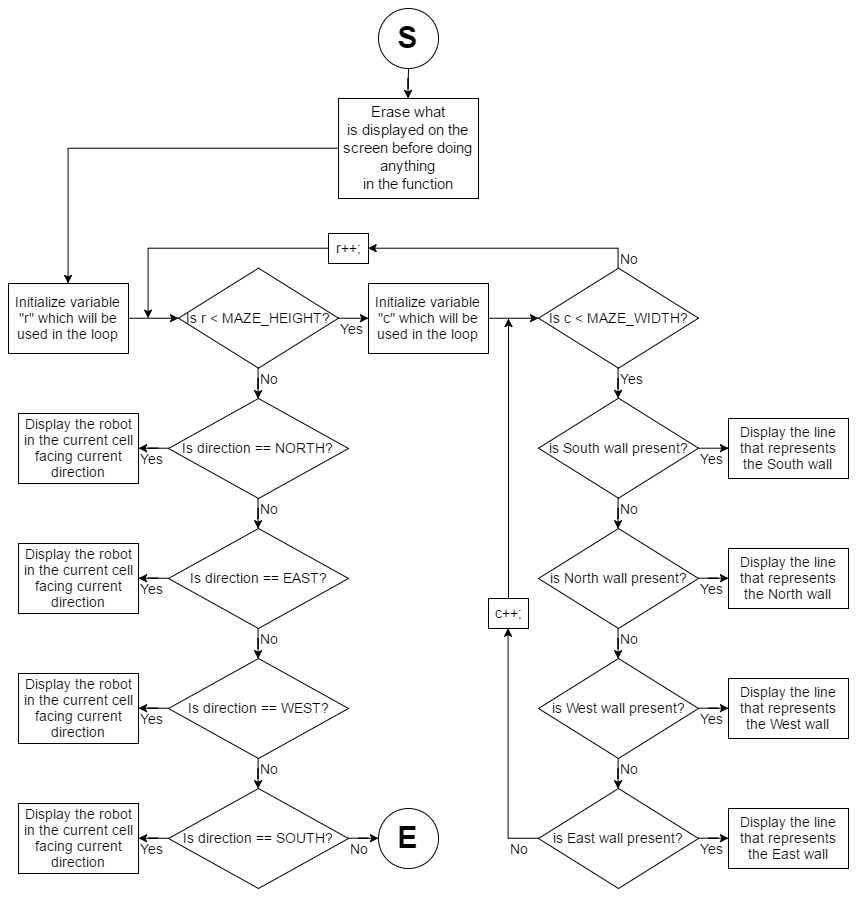
\includegraphics[scale=0.516]{images/Software_Flowchart/Drawing_Function.png}
\caption{Flow Chart for Displaying Function}
\label{}
\end{figure}
	\begin{itemize}
	\item The local variable direction is passed into the function but it does not return any variable
	\item Global variables and constants used are
	\begin{verbatim}
		MAZE_WIDTH
		MAZE_HEIGHT
		CELL_WIDTH
		CELL_HEIGHT
		CELL_WIDTH_MIDDLE
		CELL_HEIGHT_MIDDLE
	\end{verbatim}
	\end{itemize}
\end{itemize}
\newpage

%% 3.8

\subsection{Moving Forward Function}
\begin{itemize}
\item This function moves the the robot forward exactly one cell. Then, it stores the fact that there is no wall in the direction it moves. Finally, it increments how many cells it has moved without readjust. 
	\begin{verbatim}
		void goFwdCell(int direction);
	\end{verbatim}
\begin{figure}[htp]
\centering
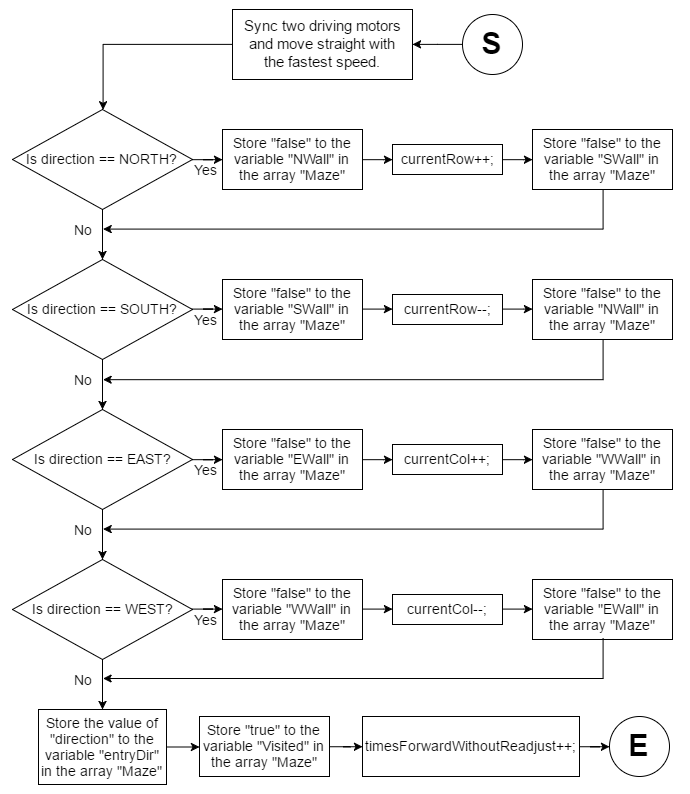
\includegraphics[scale=0.56]{images/Software_Flowchart/Moving_Forward.png}
\caption{Flow Chart for Moving Forward}
\label{}
\end{figure}	
	\begin{itemize}
	\item The local variable direction is passed into the function but it does not return any variable
	\item Global variables and constants used are
	\begin{verbatim}
		SIZE_OF_ONE_CELL
		CIRCUMFERENCE_OF_WHEEL
		DRIVE_GEAR_RATIO
		ONE_ROTATION
		FORWARD
		timesForwardWithoutReadjust
		Maze[][]
	\end{verbatim}
	\end{itemize}
\end{itemize}
\newpage

%% 3.9

\subsection{Turning Functions}
\begin{itemize}
\item Function for Turning right
\begin{verbatim}
	int Turn90CW(int direction);
\end{verbatim}
\begin{figure}[htp]
\centering
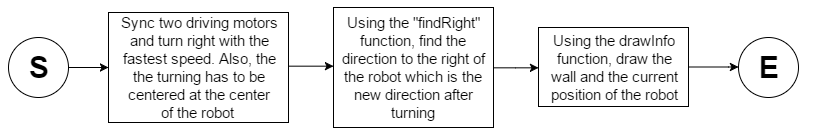
\includegraphics[scale=0.6]{images/Software_Flowchart/Turning_Right.png}
\caption{Flow Chart for Turning Right}
\label{}
\end{figure}
	\begin{itemize}
	\item The local variable direction is passed into the function and it returns the same variable direction
	\item Global variables and constants used are
	\begin{verbatim}
		QUARTER_ROTATION;
		DRIVE_GEAR_RATIO;
		FORWARD;
	\end{verbatim}
	\item This function calls in other functions
	\begin{verbatim}
		int findRight(int direction);
		int drawInfo(int direction);
	\end{verbatim}
	\end{itemize}
\item Function for Turning left 
\begin{verbatim}
	Turn90CW(int direction);
\end{verbatim}
\begin{figure}[htp]
\centering
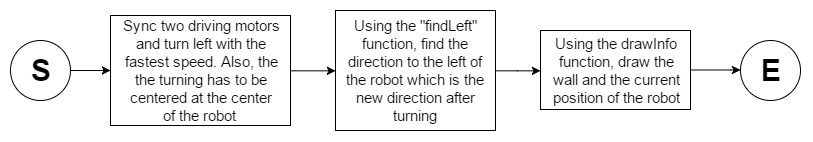
\includegraphics[scale=0.60]{images/Software_Flowchart/Turning_Left.png}
\caption{Flow Chart for Turning Left}
\label{}
\end{figure}
	\begin{itemize}
	\item The local variable direction is passes into the function and it returns the same variable direction
	\item Global variables and constants used are
	\begin{verbatim}
		QUARTER_ROTATION;
		DRIVE_GEAR_RATIO;
		FORWARD;
	\end{verbatim}
	\item This function calls in other functions
	\begin{verbatim}
		int findLeft(int direction);
		int drawInfo(int direction);
	\end{verbatim}
	\end{itemize}
\end{itemize}
\newpage

%% 3.10

\subsection{Wall Detecting Function}
\begin{itemize}
\item Function that returns whether or not there is a wall in front of the bot.
	\begin{verbatim}
		int thereIsWall();
	\end{verbatim}
\begin{figure}[htp]
\centering
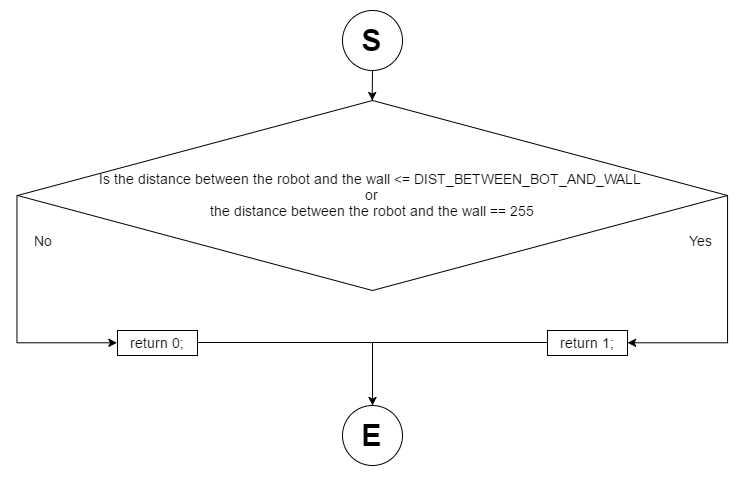
\includegraphics[scale=0.60]{images/Software_Flowchart/Detecting_Wall.png}
\caption{Flow Chart for Wall Detecting Function}
\label{}
\end{figure}
	\begin{itemize}
	\item Very simple fuction that returns $1$ if the sensor detects the wall
	\item Global variables and constants used are
	\begin{verbatim}
		DIST_BETWEEN_BOT_AND_WALL
	\end{verbatim}
	\end{itemize}
\end{itemize}
\newpage

%% 3.11

\subsection{Function for Storing Data of the Walls}
\begin{itemize}
\item Function that stores data of the walls to the variables
	\begin{verbatim}
		void writeWall(int direction);
	\end{verbatim}
\begin{figure}[htp]
\centering
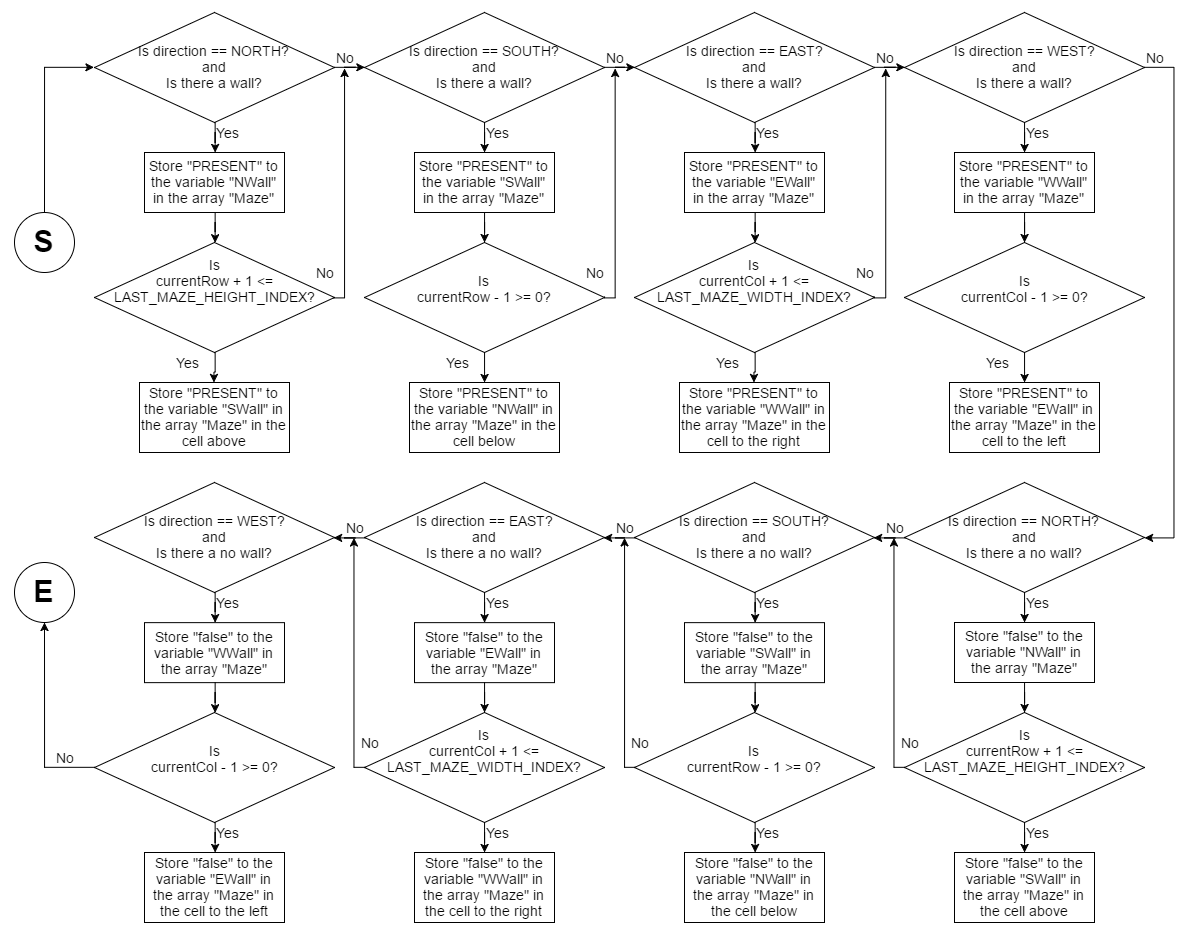
\includegraphics[scale=0.41]{images/Software_Flowchart/writeWall.png}
\caption{Flow Chart for Storing Data Function}
\label{}
\end{figure}
	\begin{itemize}
	\item The local variable direction is passed into the function but it does not return any variable.
	\item Global variables and constants used are:
	\begin{verbatim}
		NORTH
		SOUTH
		EAST
		WEST
		currentRow
		currentCol
		PRESENT
		LAST_MAZE_HEIGHT_INDEX
		LAST_MAZE_WIDTH_INDEX
	\end{verbatim}
	\item This function calls in other functions 
	\begin{verbatim}
		int thereIsWall();
	\end{verbatim}
	\end{itemize}
\end{itemize}
\newpage

%% 3.12

\subsection{Functions for setting up the direction that need to be used}
\begin{itemize}
\item Function that takes in the current direction of the robot and returns exact opposite direction of what the robot is facing
	\begin{verbatim}
		int findBackDir(int currentDirection);
	\end{verbatim}
\begin{figure}[htp]
\centering
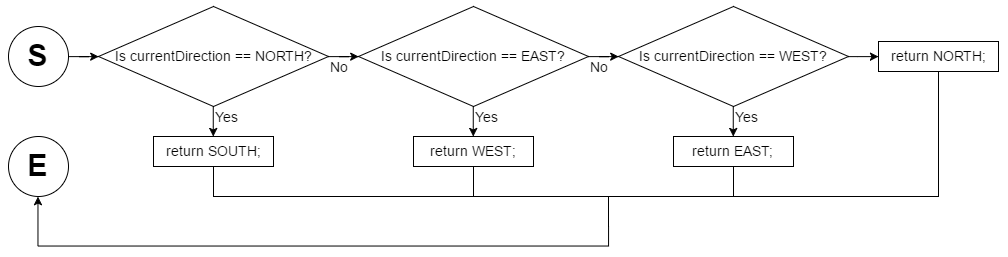
\includegraphics[scale=0.45]{images/Software_Flowchart/findBackDir.png}
\caption{Flow Chart for Finding Back Function}
\label{}
\end{figure}
\item Function that takes in a direction of the robot and returns the direction to the right of the robot.
	\begin{verbatim}
		int findRight(int currentDirection);
	\end{verbatim}
\begin{figure}[htp]
\centering
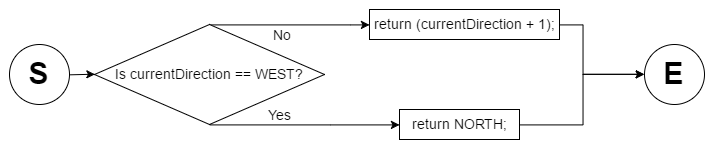
\includegraphics[scale=0.47]{images/Software_Flowchart/findRight.png}
\caption{Flow Chart for Finding Right Function}
\label{}
\end{figure}	
\item Function that takes in a direction of the robot and returns the direction to the left of the robot.
	\begin{verbatim}
		int findLeft(int currentDirection);
	\end{verbatim}
\begin{figure}[htp]
\centering
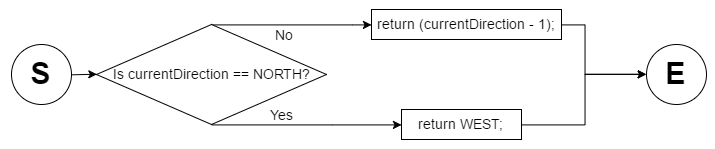
\includegraphics[scale=0.48]{images/Software_Flowchart/findLeft.png}
\caption{Flow Chart for Finding Left Function}
\label{}
\end{figure}
	\begin{itemize}
	\item Global variables and constants used are
	\begin{verbatim}
		NORTH
		SOUTH
		EAST
		WEST
	\end{verbatim}
	\end{itemize}
\end{itemize}
\newpage

%% 3.13

\subsection{Functions for Finding Existence of Wall from the data}
\begin{itemize}
\item Function takes in a direction and returns whether or not there is a wall in that direction from known data.
	\begin{verbatim}
		int isThereWallInDir(int wallDir);
	\end{verbatim}
\begin{figure}[htp]
\centering
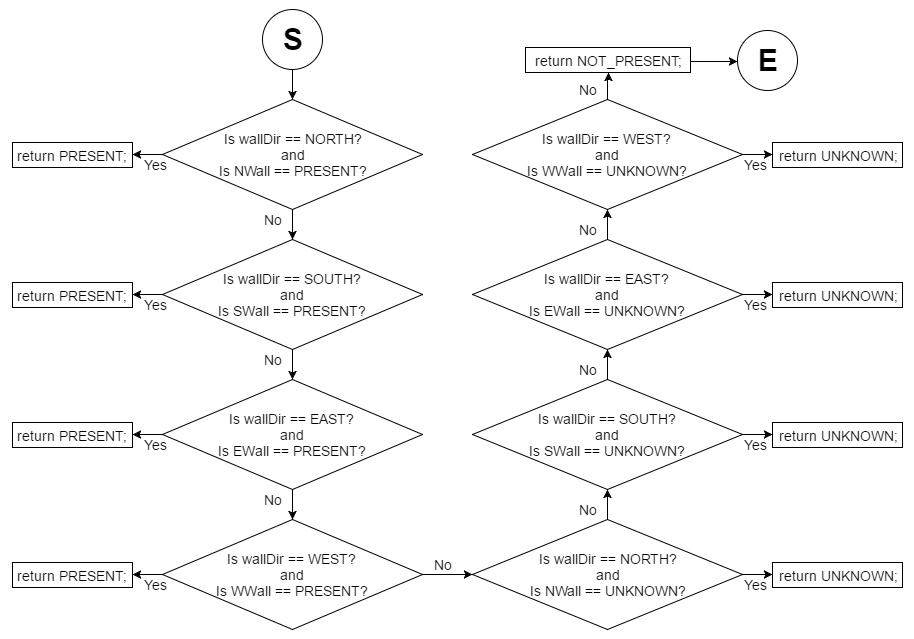
\includegraphics[scale=0.580]{images/Software_Flowchart/isThereWallInDir.png}
\caption{Flow Chart for Finding Existence of Wall from the data}
\label{}
\end{figure}
	\begin{itemize}
	\item Global variables and constants used are
	\begin{verbatim}
		NORTH
		SOUTH
		EAST
		WEST
		PRESENT
		UNKNOWN
		NOT_PRESENT
	\end{verbatim}
	\end{itemize}
\end{itemize}
\newpage

%% 3.14

\subsection{Functions for Readjusting in Certain Directions}
\begin{itemize}
\item Function that readjusts robot's position by driving into the wall and coming back to the center of the cell. For this function particularly, we readjust using walls to the front and to the right.
	\begin{verbatim}
		void reAdjustCW(int direction);
	\end{verbatim}
\begin{figure}[htp]
\centering
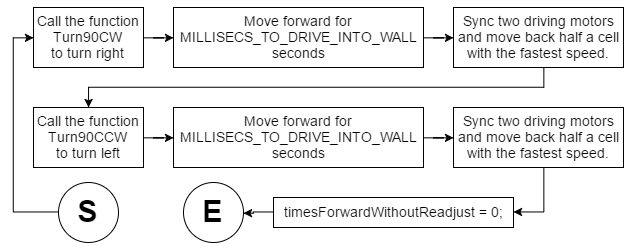
\includegraphics[scale=0.52]{images/Software_Flowchart/reAdjustCW.png}
\caption{Flow Chart for Readjusting using Front wall and Right wall}
\label{}
\end{figure}
\item Function that readjusts robot's position by driving into the wall and coming back to the center of the cell. For this function particularly, we readjust using walls to the back and to the left.
	\begin{verbatim}
		void reAdjustCCW(int direction);
	\end{verbatim}
\begin{figure}[htp]
\centering
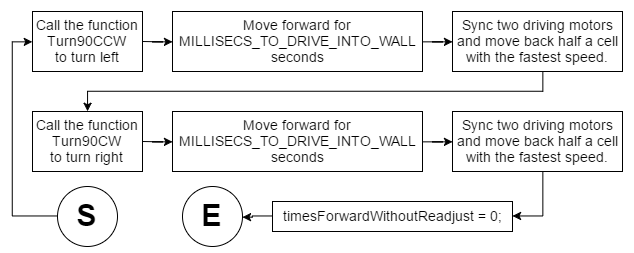
\includegraphics[scale=0.52]{images/Software_Flowchart/reAdjustCCW.png}
\caption{Flow Chart for Readjusting using Front wall and Left wall}
\label{}
\end{figure}
	\begin{itemize}
	\item The local variable direction is passed into the function but it does not return any variable
	\item Global variables and constants used are
	\begin{verbatim}
		FORWARD
		BACKWARD
		SIZE_OF_ONE_CELL
		CIRCUMFERENCE_OF_WHEEL
		DRIVE_GEAR_RATIO
		ONE_ROTATION
		UNCERTAINTY_READJUST
		MILLISECS_TO_DRIVE_INTO_WALL
	\end{verbatim}
	\item This function calls in other functions
	\begin{verbatim}
		int Turn90CW(int direction);
		int Turn90CCW(int direction);
	\end{verbatim}
	\end{itemize}
\newpage
\item Function that decides which direction to readjust in using the data collected in array. Once the function decides the direstion to readjust in, it cals that function.
	\begin{verbatim}
		void reAdjustWayBack(int direction);
	\end{verbatim}
\begin{figure}[htp]
\centering
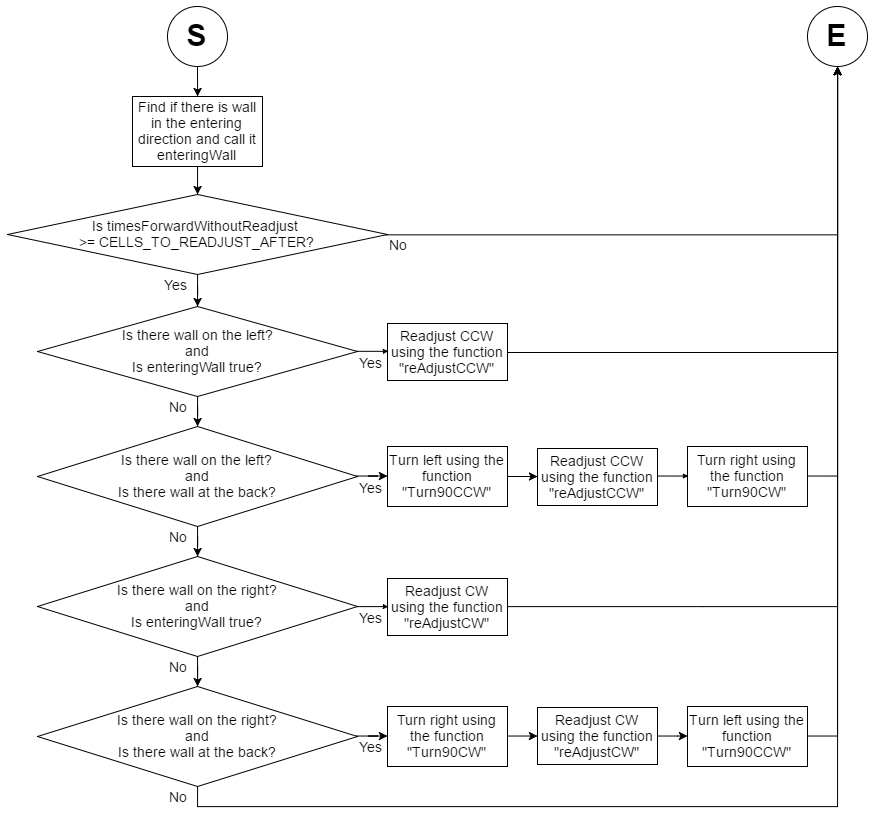
\includegraphics[scale=0.46]{images/Software_Flowchart/reAdjustWayBack.png}
\caption{Flow Chart for Readjusting using walls detected}
\label{}
\end{figure}
	\begin{itemize}
	\item The local variable direction is passed into the function but it does not return any variable
	\item Global variables and constants used are
	\begin{verbatim}
		timesForwardWithoutReadjust
		CELLS_TO_READJUST_AFTER
		PRESENT
	\end{verbatim}
	\item This function calls in other functions
	\begin{verbatim}
		thereIsWall();
		reAdjustCW(int direction);
		reAdjustCCW(int direction);
		findLeft(int currentDirection);
		findRight(int currentDirection);
		findBackDir(int currentDirection);
		isThereWallInDir(int wallDir);
	\end{verbatim}
	\end{itemize}
\end{itemize}
\newpage

%% 3.15

\subsection{Function for Movement All Together}
\begin{itemize}
\item Function that implements the right following algorithm using the functions described above. Furthermore, ensures that the robot readjusts whenever it can.
	\begin{verbatim}
		int MovementWithSensor(int direction);
	\end{verbatim}
\begin{figure}[htp]
\centering
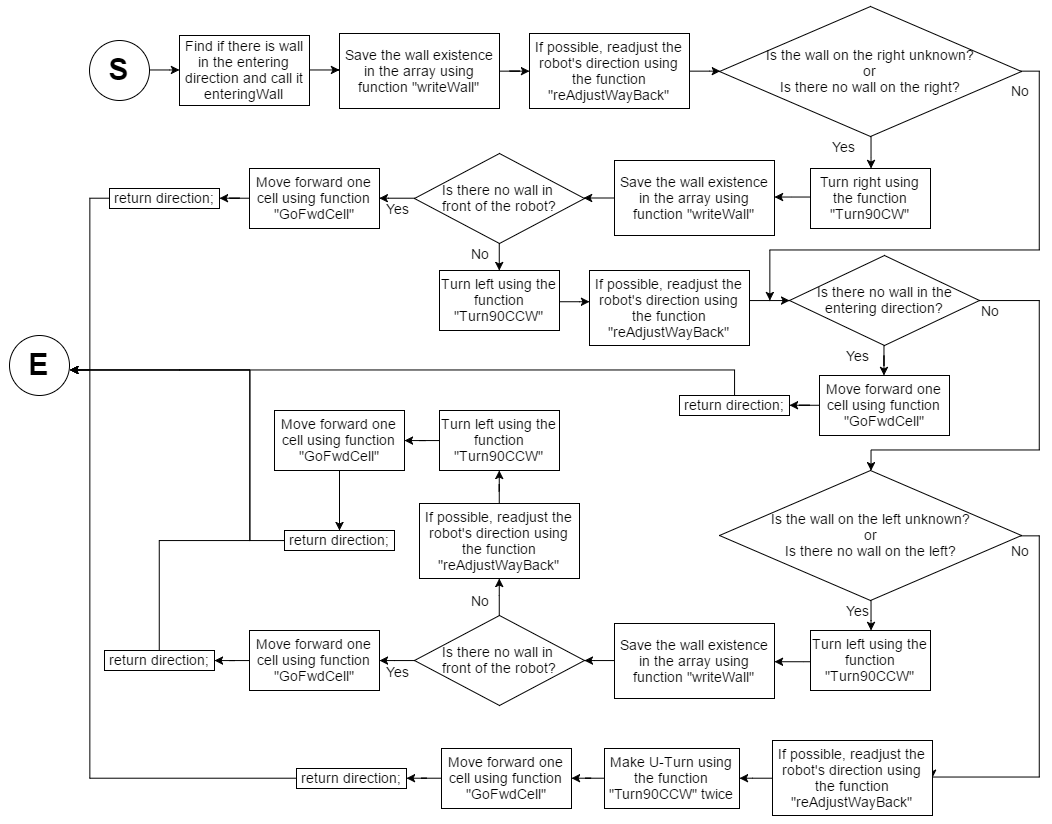
\includegraphics[scale=0.45]{images/Software_Flowchart/MovementWithSensor.png}
\caption{Flow Chart for Movement Function}
\label{}
\end{figure}
	\begin{itemize}
	\item The local variable direction is passed into the function and it returns a new variable direction.
	\item Global variables and constants used are
	\begin{verbatim}
		UNKNOWN
		NOT_PRESENT
	\end{verbatim}
	\item This function calls the other functions
	\begin{verbatim}
		writewall(int direction);
		reAdjustWayBack(int direction);
		isThereWallInDir(int wallDir);
		findRight(int currentDirection);
		thereIsWall();
		goFwdCell(int direction);
		Turn90CCW(int direction);
		Turn90CW(int direction);
	\end{verbatim}
	\end{itemize}
\end{itemize}
\newpage

%% 3.16

\subsection{Functions for Returning Algorithm}
\begin{itemize}
\item Function that deletes the duplicates from the array which saved up how the robot entered each cell. For example, if the robot moved two opposite directions in order, it is not necessary. Therefore, we delete the duplicates from the array
 	\begin{verbatim}
		void deleteDuplicates();
	\end{verbatim}
\begin{figure}[htp]
\centering
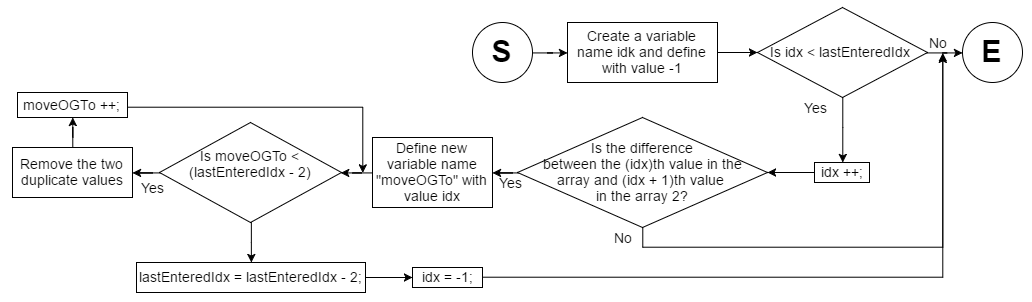
\includegraphics[scale=0.50]{images/Software_Flowchart/deleteDuplicate.png}
\caption{Flow Chart for Deleting Duplicate Function}
\label{}
\end{figure}
\item Function that reverses the direction from the array which saved up how the robot entered each cell. For example, if the robot went into the cell with direction East, then we change it to West. Therefore, we change all the directions to its opposite.
 	\begin{verbatim}
		void reverseDirection();
	\end{verbatim}
\begin{figure}[htp]
\centering
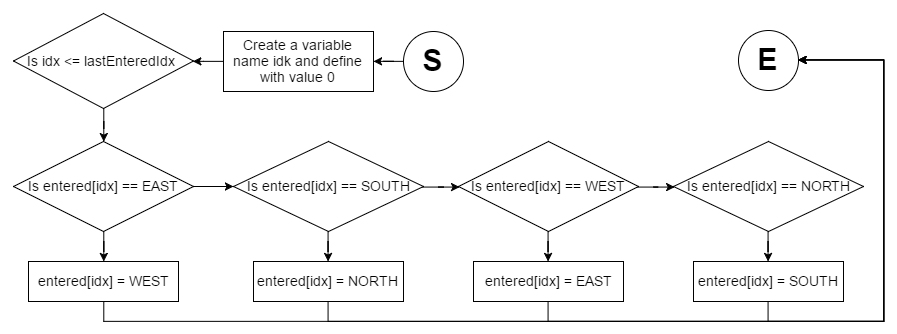
\includegraphics[scale=0.50]{images/Software_Flowchart/reverseDirection.png}
\caption{Flow Chart for Reversing Order of Values in the Array}
\label{}
\end{figure}
\newpage
\item Function that takes in the variable direction and goes back to the initial position in the cell with the new array created by two functions above
 	\begin{verbatim}
		void goingBackFastestRoute(int direction);
	\end{verbatim}
\begin{figure}[htp]
\centering
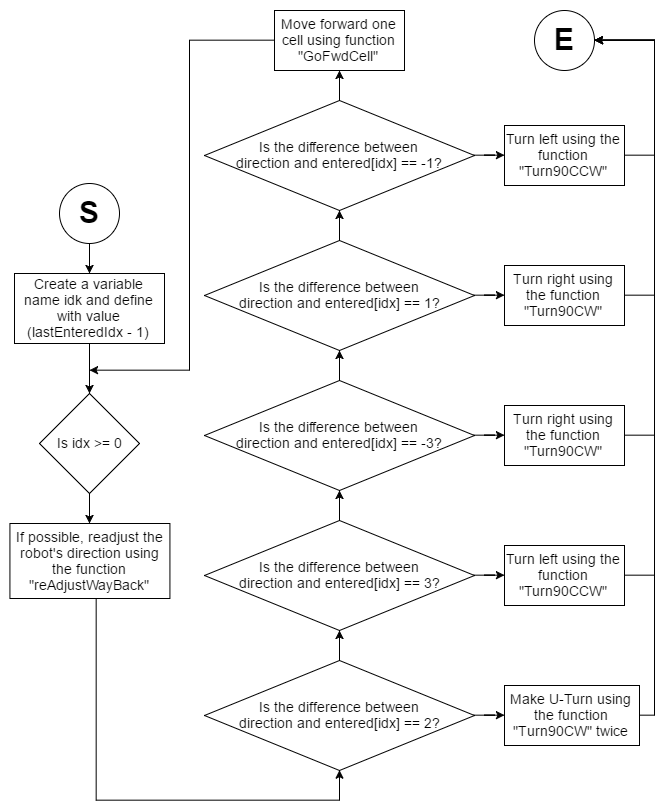
\includegraphics[scale=0.53]{images/Software_Flowchart/goingBackFastestRoute.png}
\caption{Flow Chart for Function to Go Back to Initial Position}
\label{}
\end{figure}
	\begin{itemize}
	\item Global variables and constants used are
	\begin{verbatim}
		lastEnteredIdx
		EAST
		WEST
		SOUTH
		NORTH
	\end{verbatim}
	\item This function calls in other functions
	\begin{verbatim}
		reAdjustWayBack(int direction);	
		Turn90CW(int direction);
		Turn90CCW(int direction);
	\end{verbatim}
	\end{itemize}
\end{itemize}
\newpage

%% 3.17

\subsection{Main Function}
\begin{itemize}
\item More than ten functions were declared for simplicity of the main function. This function sums up all smaller functions
	\begin{verbatim}
		task main()
	\end{verbatim}

	\begin{itemize}
	\item A variable that represents current direction of the robot was declared. This is initialized as north as this is the orientation of the robot when it first enters the maze.
	\begin{verbatim}
		int direction = NORTH;
	\end{verbatim}
	
	\item Global variables and constants used are
	\begin{verbatim}
		MAZE_WIDTH
		MAZE_HEIGHT
		UNKNOWN
		PRESENT
		lastEnteredIdx
		FREQUENCY
		MILI_TO_BEEP_FOR
	\end{verbatim}
	\item This function calls in other functions
	\begin{verbatim}
		MovmentWithSensor(int direction);
		deleteDuplicates();
		reverseDirection();
		goingBackFastestRoute(int direction);
		drawInfo(int direction);
	\end{verbatim}
	\end{itemize}
 

\end{itemize}
Flow chart is on the next page.

\begin{figure}[htp]
\centering
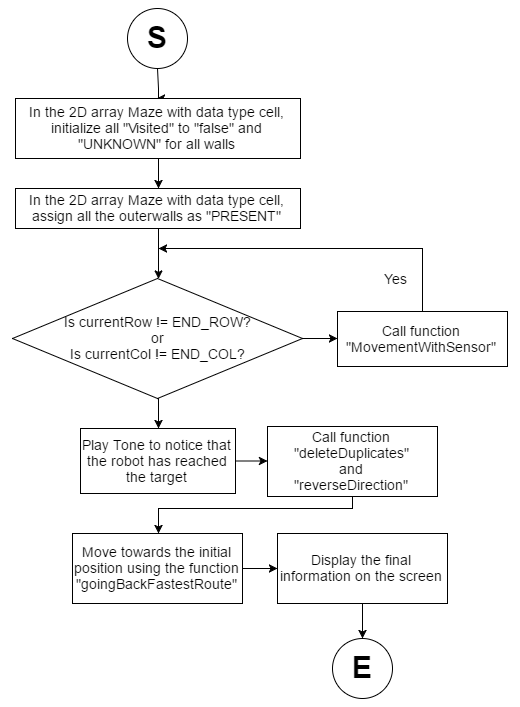
\includegraphics[scale=0.51]{images/Software_Flowchart/task_main.png}
\caption{Flow Chart of the Main Function}
\label{}
\end{figure}
\newpage

%% Do not remove the gap %%








\section{Appendix}

Source of Code with brief comments


\end{document}
